\chapter{Introducción}\label{cap.introduccion}
El Trabajo Fin de Grado (TFG) descrito a continuación se encuadra en el entorno educativo \textit{Robotics-Academy}, para la enseñanza de la programación de robots. La intención principal de su desarrollo es extender este entorno docente con nuevos ejercicios que representen problemas atractivos en la robótica. En este capítulo se introducirá el contexto en el que se sitúa este proyecto y la motivación que he llevado a su desarrollo. Es preciso comenzar con una explicación a grandes rasgos sobre qué es la robótica y sus aplicaciones en la sociedad.

La parte más importante de la inteligencia de los robots viene suministrada por el software. Dentro del software destacaremos diferentes elementos como los simuladores, las bibliotecas de código y los middlewares de robótica. Dentro de la robótica, el contexto concreto relacionado con este TFG es la robótica educativa, y en particular, el propio entorno \textit{Robotics-Academy}, desarrollado en la Universidad Rey Juan Carlos.

\section{Robótica}
A lo largo de la historia, la ciencia y la tecnología han sido utilizadas por el hombre para facilitarle la vida. Para ello, ha ideado, desarrollado y construido herramientas y máquinas empleándolas para reducir su carga de trabajo. La robótica es la rama de la tecnología basada en la utilización de la informática para el diseño y desarrollo de sistemas automáticos que faciliten la vida al ser humano e, incluso, llegan a sustituirle en algunas tareas determinadas. La robótica incluye conceptos de disciplinas diversas, como la física, las matemáticas, la electrónica, la mecánica, la inteligencia artificial, la ingeniería de control, etc. Gracias a todas estas disciplinas involucradas unidas convenientemente se pueden diseñas máquinas que ejecuten comportamientos autónomos según el propósito para el que han sido desarrolladas. Estas máquinas autónomas se denominan "Robots".

Desde 1950, estos sistemas autónomos han experimentado un crecimiento exponencial en cuanto a complejidad, versatilidad, autonomía y, sobre todo, en su incorporación a una gran diversidad de ámbitos. Los sistemas operados por el ser humano comienzan a incorporar un sistema de control específico programable que permiten el desarrollo de tareas repetitivas o con un gran riesgo para las personas, englobando tareas básicas y de difícil realización, hasta la actualidad, en la cual existe un gran marco de ejemplos en los que se integran la robótica y multitud de campos y tareas. Los robots comerciales e industriales realizan las tareas de una manera más exacta o más barata que las personas. También son utilizados en trabajos peligrosos, sucios tediosos para el ser humano. Gracias a esto, se trata de un campo en crecimiento constante.

\begin{figure}[H]
	\begin{center}
		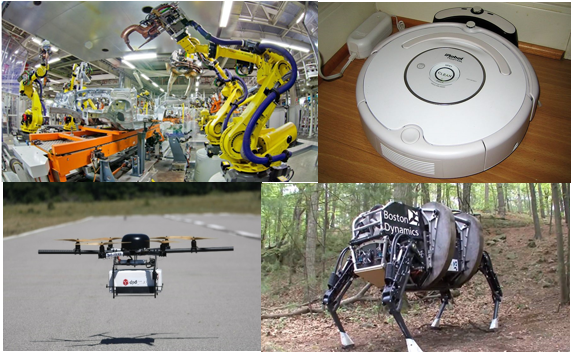
\includegraphics[width=0.8\textwidth]{figures/robots.png}
		\caption{Robots modernos}
		\label{fig.robots}
	\end{center}
\end{figure}

Ya se ha comentado la importancia de los robots en la actualidad en el aspecto industrial, pero tal el crecimiento que está experimentando la robótica que está comenzando a cobrar una gran importancia en aspectos menos especializados como el entorno doméstico. Cabe destacar el desarrollo de robots para facilitar la vida al ser humano, un ejemplo está ilustrado en la Figura 1.1. Las aspiradoras robóticas (Roomba, Dyson, Xiami, ...) han tenido un éxito rotundo en la realización de una actividad doméstica necesaria para la vida del ser humano.

Otro éxito de la robótica en la actualidad es el desarrollo de coches autónomos. Este hecho se ha conseguido paulatinamente mediante la incorporación de tecnología cada vez más sofisticada a los automóviles. En este aspecto cabe destacar los módulos de aparcamiento automático, el park assist o los asistentes de conducción autónoma (autopiloto Tesla), o los prototipos de coches autónomos (Apple o Google). 
Otro ámbito en el que la robótica ha sido introducida es el militar, donde se han incorporado robots de rescate o para la desactivación de bombas. 

En la medicina se ha desarrollado el robot DaVinci (Figura \ref{fig.DaVinci}), que permite operar desde cualquier parte del mundo con una precisión mayor a la humana. En el ámbito de la logística Amazon ha desarrollado una flota de robots de almacén que consiguen trasladar los pedidos a lo largo de sus almacenes (Figura \ref{fig.Amazon}). Tal es el punto de crecimiento de la robótica que se están desarrollando robots con ``comportamientos inteligentes'' como el robot Atlas de \textit{Boston Dynamics} (Figura \ref{fig.Atlas}) que pueden interactuar con humanos, ya sea como asistente para el hombre o con fines experimentales como la locomoción bípeda.

\begin{figure}[H]
	\centering
	\begin{minipage}[h]{.48\linewidth}
		\centering
		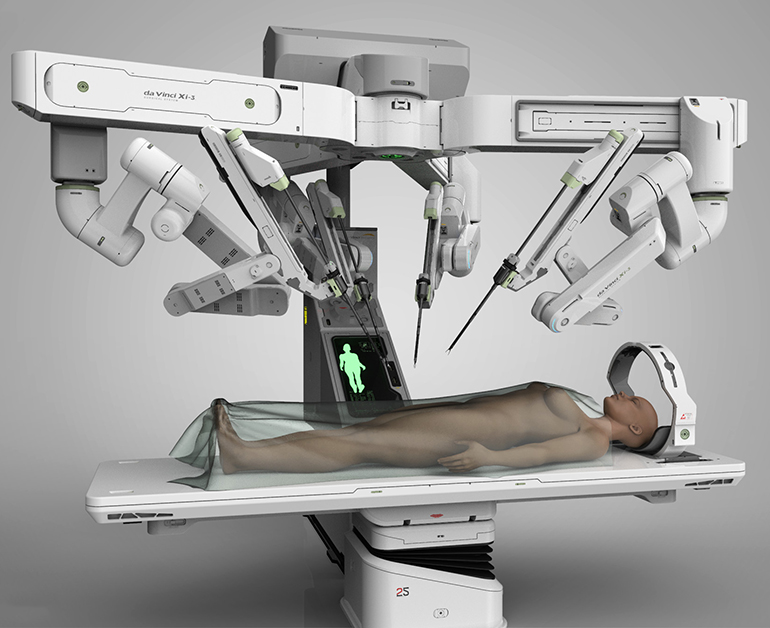
\includegraphics[width=.9\linewidth, height=7cm]{figures/DaVinci.jpg}
		\captionof{figure}{Robot DaVinci}
		\label{fig.DaVinci}
	\end{minipage}
	\begin{minipage}[h]{.48\linewidth}
		\centering
		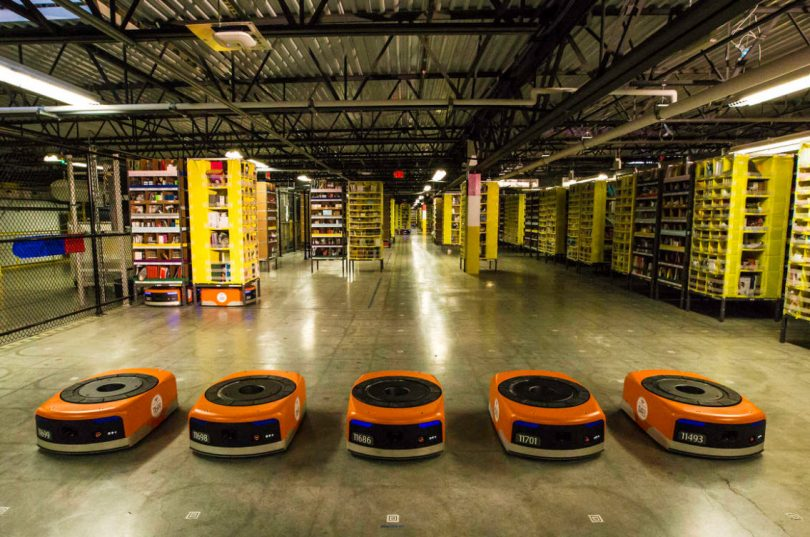
\includegraphics[width=.9\linewidth, height=7cm]{figures/Amazon.jpg}
		\captionof{figure}{Flota de robot de Amazon}
		\label{fig.Amazon}
	\end{minipage}
\end{figure}

\begin{figure}[H]
    \begin{center}
        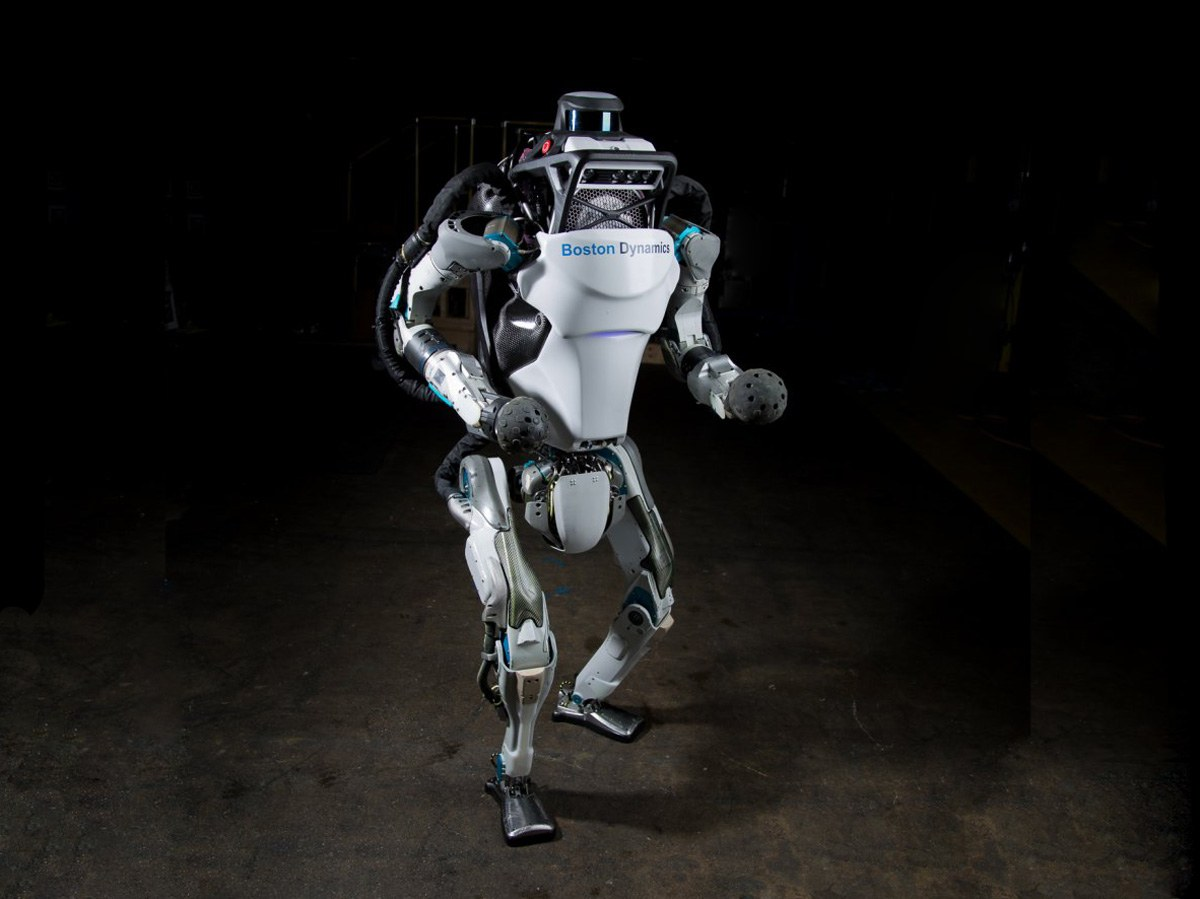
\includegraphics[width=.7\linewidth, height=7cm]{figures/BDY_Atlas.jpg}
		\captionof{figure}{Robot Atlas}
		\label{fig.Atlas}
    \end{center}
\end{figure}

Los ámbitos de aplicación de la robótica son cada vez más extensos gracias al auge de esta ciencia. Algunos ejemplos son la agricultura de precisión mediante drones con análisis de imágenes térmicas y multiespectral para aumentar el rendimiento de las explotaciones agrícolas o el control de los productos industriales mediante el procesado de imágenes de la producción o la automatización de aplicaciones anestésicas de bajo nivel e, incluso, competiciones deportivas de robots.

\section{Software Robótico}
Para que los robots puedan ser controlados de una manera eficaz el comportamiento del software que los controla debe ser robusto. Para ello, el \textit{software} de la robótica, se divide en distintas capas (\textit{drivers}, \textit{middleware} y aplicaciones), cuya arquitectura será distinta, típicamente, según su aplicación final.

Debido al gran desarrollo de la robótica, los robots actuales ya no precisan del control del ser humano para su funcionamiento, en la actualidad tienen comportamientos autónomos que les permiten realizar las tareas sin la mediación de terceros. Esto es posible gracias al minucioso desarrollo del software que compone los sistemas complejos del robot, algo parecido a una inteligencia autónoma. El desarrollo del software robótico parte de ciertas tareas o requisitos como son los circuitos de retroalimentación, control, búsqueda de caminos, localización o filtrado de datos entre otras muchas.

En los últimos años se han creado una gran cantidad de plataformas de desarrollo de software para las aplicaciones robóticas, también llamados \textit{middleware} robóticos. Los simuladores son otra herramienta importante para el desarrollo de software robótico ya que permiten realizar pruebas y depurar los fallos para programar una versión funcional del robot antes de ser fabricado. 

\subsection{Middlewares robóticos}
Los \textit{middleware} robóticos pueden definirse como entornos o \textit{frameworks} para el desarrollo de software pare robots. Se trata de software que conecta aplicaciones o componentes software para soportar aplicaciones complejas y distribuidas. Para controlar los sensores y actuadores de los robots estos entornos incluyen \textit{drivers}, arquitectura software para las aplicaciones que se van a crear, bloques de funcionalidad robótica ya resuelta, además de simuladores, visualizadores... Por ello al \textit{middleware} se le suele conocer como "pegamento para software". Una de las tareas del \textit{middleware} es conectar el hardware, ya sea real o simulado, con la aplicación desarrollada. El \textit{middleware} más extendido en el mundo es ROS.

\textbf{Robot Operating System (ROS)\footnote{\url{http://www.ros.org/}}} es una plataforma de software libre para el desarrollo software de robots que proporciona la funcionalidad de un sistema operativo en un clúster heterogéneo como el control de dispositivos de bajo nivel, mecanismos de intercambio de mensajes entre procesos y la abstracción del hardware, necesarios para el desarrollo de la robótica. Aunque el \textit{framework} ROS se desarrolló para los sistemas UNIX, se ha adaptado para ser soportado en otros sistemas operativos como Fedora, Debian, Windows, Mac OS X, Arch, Slackware, Gento u OpenSUSE, llegando a permitir las aplicaciones multiplataforma. Gracias a esto el \textit{framework} ROS se ha convertido en el más utilizado.

Existen otros \textit{framework} interesantes como \textbf{Orocos}\footnote{\url{http://www.orocos.org/}} que permite el control avanzado de máquinas y robots en C++, \textbf{Orca}\footnote{\url{http://orca-robotics.sourceforge.net//}} que está orientado a componentes por lo que permite el desarrollo de aplicaciones más complejas y de \textit{software} libre y \textbf{Urbi}\footnote{\url{https://github.com/urbiforge/urbi}} que es un \textit{middleware} multiplataforma de código abierto en C++ que permite desarrollar aplicaciones en sistemas completos y complejos y rabaja de forma conjunta con ROS.

\subsection{Simuladores robóticos}
Debido al gran coste que supone la fabricación del hardware del robot es preciso depurar los posibles errores que contenga el código, así como el funcionamiento del hardware antes de su fabricación. Por ello debe probarse el código en un simulador orientado al tipo de aplicación que estemos desarrollando. Gracias a los simuladores es posible probar este código sin tener que fabricar previamente el hardware. De esta manera cualquier mal funcionamiento del código del robot puede ser solventado evitando la rotura del hardware. Algunos de los simuladores más utilizados son:

\textbf{Gazebo}\footnote{\url{http://gazebosim.org/}}. Se trata del simulador 3D de código abierto más extendido. Funciona bajo la licencia Apache 2.0 y tienen gran importancia su motor de renderizado avanzado, sus motores de física y su soporte para \textit{plugins} de robot y sensores, además de su amplio catálogo de robots con sus sensores y actuadores. Otro hecho importante es su soporte para ROS lo que permite probar el código real del robot n el simulador.

\textbf{Stage}\footnote{\url{http://wiki.ros.org/stage}}. Es un simulador en dos dimensiones, integrable con ROS, que permite simular numerosos robots simultáneamente.

\textbf{Webots}\footnote{\url{https://www.cyberbotics.com/}}. Simulador de robótica avanzada en el que se pueden desarrollar modelos propios y su física, escribir sus controladores y hacer simulaciones a gran velocidad. Un ejemplo es su soporte para el humanoide Nao. Actualmente, se ha convertido en \textit{software} libre.

\section{Docencia en robótica}
La robótica con fines educativos está adquiriendo gran importancia en la actualidad en la enseñanza preuniversitaria. Esto es debido a que su aprendizaje está disponible para estudiantes de cualquier nivel, el único requisito para estudiar robótico es la motivación por el desarrollo de aplicaciones. La robótica en el campo de la docencia resulta especialmente interesante al ser una ciencia multidisciplinar, muy relacionada con campos multidisciplinares como electrónica, informática, mecánica, física, ... Gracias a ello el estudiante adquiere una gran variedad de conocimiento de todas estas áreas.

En docencia primaria y secundaria se intenta despertar el interés del estudiante por la robótica, con la transformación de asignaturas teóricas tradicionales en asignaturas más prácticas e interactivas, ya que la robótica permite la recreación de problemas que les rodean y a través de los cuales pueden utilizar su creatividad y plasmar los conceptos teóricos que han adquirido.
En los centros de enseñanza primaria y secundaria se imparte robótica mediante plataformas físicas como los robots LEGO (Mindstorms, RCX, NXT, Evo, WeDo), placas Arduino, los kits de SolidWorks, etc.

En la docencia universitaria se imparte la robótica en distintos Grados y Postgrados en las escuelas de ingeniería. En España, se puede cursar la docencia robótica en el ``Grado en Ingeniería Robótica'' de la Universidad de Alicante, en los Grados de ``Electrónica Industrial y Automática'' o ``Ingeniería Electrónica, Robótica y Mecatrónica'' en distintas universidades, además de grados como el ``Grado en Ingeniería Robótica Software'' que imparte la Universidad Rey Juan Carlos desde el mes de Septiembre. Sin embargo, la docencia en robótica se reserva mayoritariamente para los Postgrados, dado que se trata una disciplina muy especializada. Existen varios Másteres destacados relacionados con la docencia de robótica como el ``Máster de Visión Artificial'', el ``Máster Universitario en Ingeniería Mecatrónica'', o el ``Máster Universitario en Automática y Robótica''.

Dentro del ámbito internacional pueden encontrarse distintas universidades que destacan en robótica como el MIT, Carnegie Mellon University, Standford o Geordia Institute of Technology. También existen asociaciones prestigiosas como ACM (Association for Computing and Machinery) y la IEEE-CS (IEEE Computer Society) que ven la robótica como una ciencia imprescindible en estudios de ingeniería, informática y sistemas inteligentes.

\subsection{Robotics-Academy}
En cuanto a la propia Universidad Rey Juan Carlos, cuenta con la plataforma software JdeRobot, que consta de un entorno académico para la docencia de robótica llamado Robotics-Academy. Este entorno educativo se ha utilizado con éxito en distintas asignaturas como ``Visión en Robótica'' del Máster de Visión Artificial o en la asignatura Robótica del Grado de Ingeniería Telemática. También se ha usado en cursos de programación de drones y de robótica para estudiantes universitarios.

Con este trabajo se ha pretendido extender las posibilidades de aprendizaje en este entorno, ampliándolo con dos nuevos ejercicios.
Los ejes en los que se apoya Robotics-Academy son:
\begin{enumerate}[label=\alph*)]
	\item Lenguaje Python (por su sencillez y potencia).
	\item Simulador Gazebo (con distintos modelos de robot, tales como drones, formula1, brazos, aspiradoras, etc.).
	\item Foco en el algoritmo en vez de en el middleware, ocultando al estudiante los detalles de la infraestructura.
\end{enumerate}

Debido a la compatibilidad de JdeRobot con ROS y Gazebo, se pueden utilizar los \textit{plugins} de ROS para las simulaciones en Gazebo de las prácticas presentes en el entorno Robotics-Academy mediante el establecimiento de las conexiones de los sensores y actuadores de la práctica con los \textit{plugins} de ROS en el nodo académico de la misma.

El entorno Robotics-Academy cuenta con elenco de prácticas que abordan distintos problemas clásicos de la robótica. Para cada práctica se dispone de una plantilla que resuelve tareas auxiliares como la conexión con sensores y actuadores necesarios, la temporización o la interfaz gráfica y aloja el código del algoritmo del estudiante. De esta manera el estudiante se puede centrar en la solución del ejercicio exclusivamente. Cada plantilla está formado por una parte específica oculta y el algoritmo con la lógica del robot del estudiante que se rellena en un fichero.

Debido a esta estructura, pueden distinguirse distintas capas en la composición de la práctica. La capa de nivel más bajo se le facilita al estudiante que sólo se centra en la capa superior donde se aloja la lógica del robot. Aunque esta capa más baja le viene dada al estudiante, es necesaria su implementación para dar solución a la práctica.Se incluyen las conexiones de los sensores y actuadores del robot, la interfaz gráfica, la temporización, el desarrollo del modelo del robot y un escenario que lo contenga, los plugins del modelo, los \textit{drivers} del mismo y la comunicación entre el simulador y el componente académico de alto nivel. Todo esto puede apreciarse en la Figura \ref{fig.estructura}:

\begin{figure}[H]
  \begin{center}
    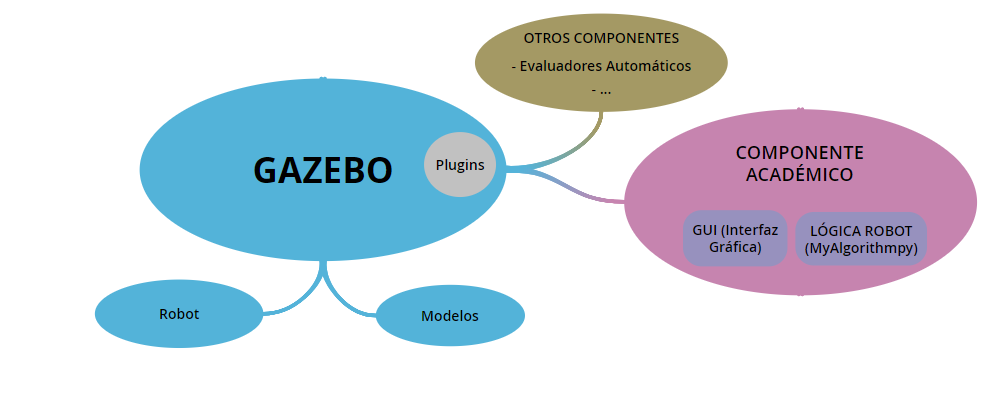
\includegraphics[width=0.9\linewidth]{figures/estructura_jde.png}
		\caption{Estructura de una práctica en Robotics-Academy}
		\label{fig.estructura}
		\end{center}
\end{figure}

Se puede apreciar que la arquitectura software de las prácticas académicas facilita el desarrollo de las mismas por parte de los alumnos de manera que sólo se concentran en el desarrollo del algoritmo con la lógica del robot.

El entorno usual para la realización de las prácticas es el simulador Gazebo, aunque las prácticas se han desarrollado de manera que puedan ser ejecutadas en robots reales sin realizar ninguna modificación, con los correspondientes drivers del robot. Gracias a esto, el código puede ser probado en robots reales. El sistema operativo base sobre el que se han desarrollado todo el entorno educativo.

\subsubsection{ Plantilla como nodo ROS}
Una de las posibilidades que ofrece este entorno educativo para realizar los problemas que ofrece es mediante los nodos ROS. De esta manera, basta con instalar el paquete de la plataforma y se puede acceder a cualquiera de las prácticas que lo componen, además de tener todas las herramientas necesarias para su desarrollo.

 El componente académico es el encargado de conectar el  con el código desarrollado por el alumno desde el fichero \textit{MyAlgorithm.py} y visualizar trazas que ayuden a la depuración del código, como las imágenes procesadas, datos del láser o imágenes de la cámara integrada, dependiendo de la práctica.

\subsubsection{Plantilla con cuadernillos de Jupyter}
También se puede acceder a las prácticas docentes con el navegador web. De esta manera se convierte al entorno Robotics-Academy en multiplataforma, dotándolo de mayor accesibilidad. Esto es gracias al desarrollo de la interfaz web de Gazebo para la simulación, a la plataforma \textit{Jupyter} (ver \ref{cap.Jupyter}) que, mediante sus cuadernillos, han permitido trasladar las prácticas de Robotics-Academy a ellos.

Esta versión web de Robotics-Academy proporciona un servidor remoto para el desarrollo y ejecución de las prácticas. Esto supone una gran innovación y el paso final al soporte multiplataforma del entorno docente.

Para ello, se basa en el uso de Jupyter para cargar el cuadernillo académico de las prácticas, así como de un script (incluido en el \textit{Notebook} de Jupyter) para realizar las conexiones de los sensores y actuadores del robot con el nodo académico. También utiliza el soporte del simulador Gazebo en navegadores web para ofrecer una visualización del escenario de la práctica cargando un fichero \textit{.world} donde se incluye la descripción del robot y el mundo. 

Para soportar esta carga computacional, el servidor de la plataforma está basado en el servidor \textit{Apache}\footnote{\url{https://www.apache.org/}}, sobre el que se ha desarrollado un servidor en \textit{Django}\footnote{\url{https://www.djangoproject.com/}}. Ambas plataformas son de código libre y proporcionan el código necesario para el desarrollo de servidores web. Por último, utiliza \textit{Dockers}\footnote{\url{https://www.docker.com/}} para ofrecer al estudiante todos los componentes necesarios para dar soporte a toda la infraestructura anterior. De esta manera, ROS-Kinetic, modelos, escenarios, \textit{plugins}, \textit{drivers}, etc, se usan y son totalmente transparentes al alumno.

Mediante la integración de toda esta infraestructura se ha desarrollado  una página y servidor web \textit{Academy-Web} que proporciona al estudiante todas las herramientas necesarias para realizar las prácticas de una manera muy sencilla. El servidor ofrece la visualización del escenario en Gazebo junto con el cuadernillo de \textit{Jupyter} en el que está presente la celda en la que el estudiante desarrollará su código.

\begin{figure}[H]
  \begin{center}
    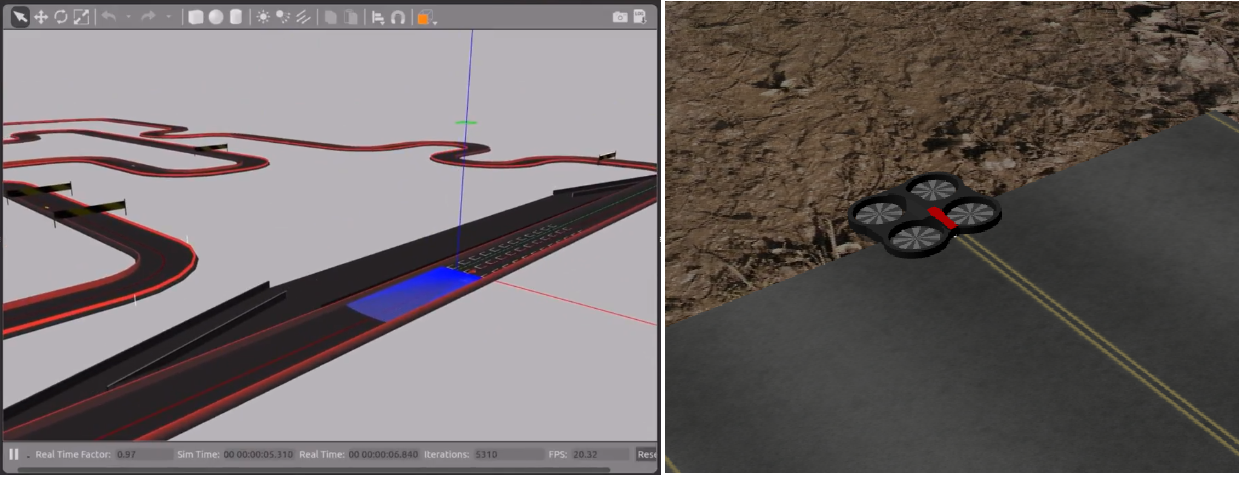
\includegraphics[width=0.9\linewidth]{figures/gazeboworlds.png}
		\caption{Visualización de las prácticas ``Follow Line'' y ``Follow Road'' en la versión web de Robotics-Academy}
		\label{fig.academyweb}
		\end{center}
\end{figure}

\subsubsection{Ejercicios disponibles}
Algunas de las prácticas que componen la plataforma son las siguientes:

\begin{figure}[H]
  \begin{center}
    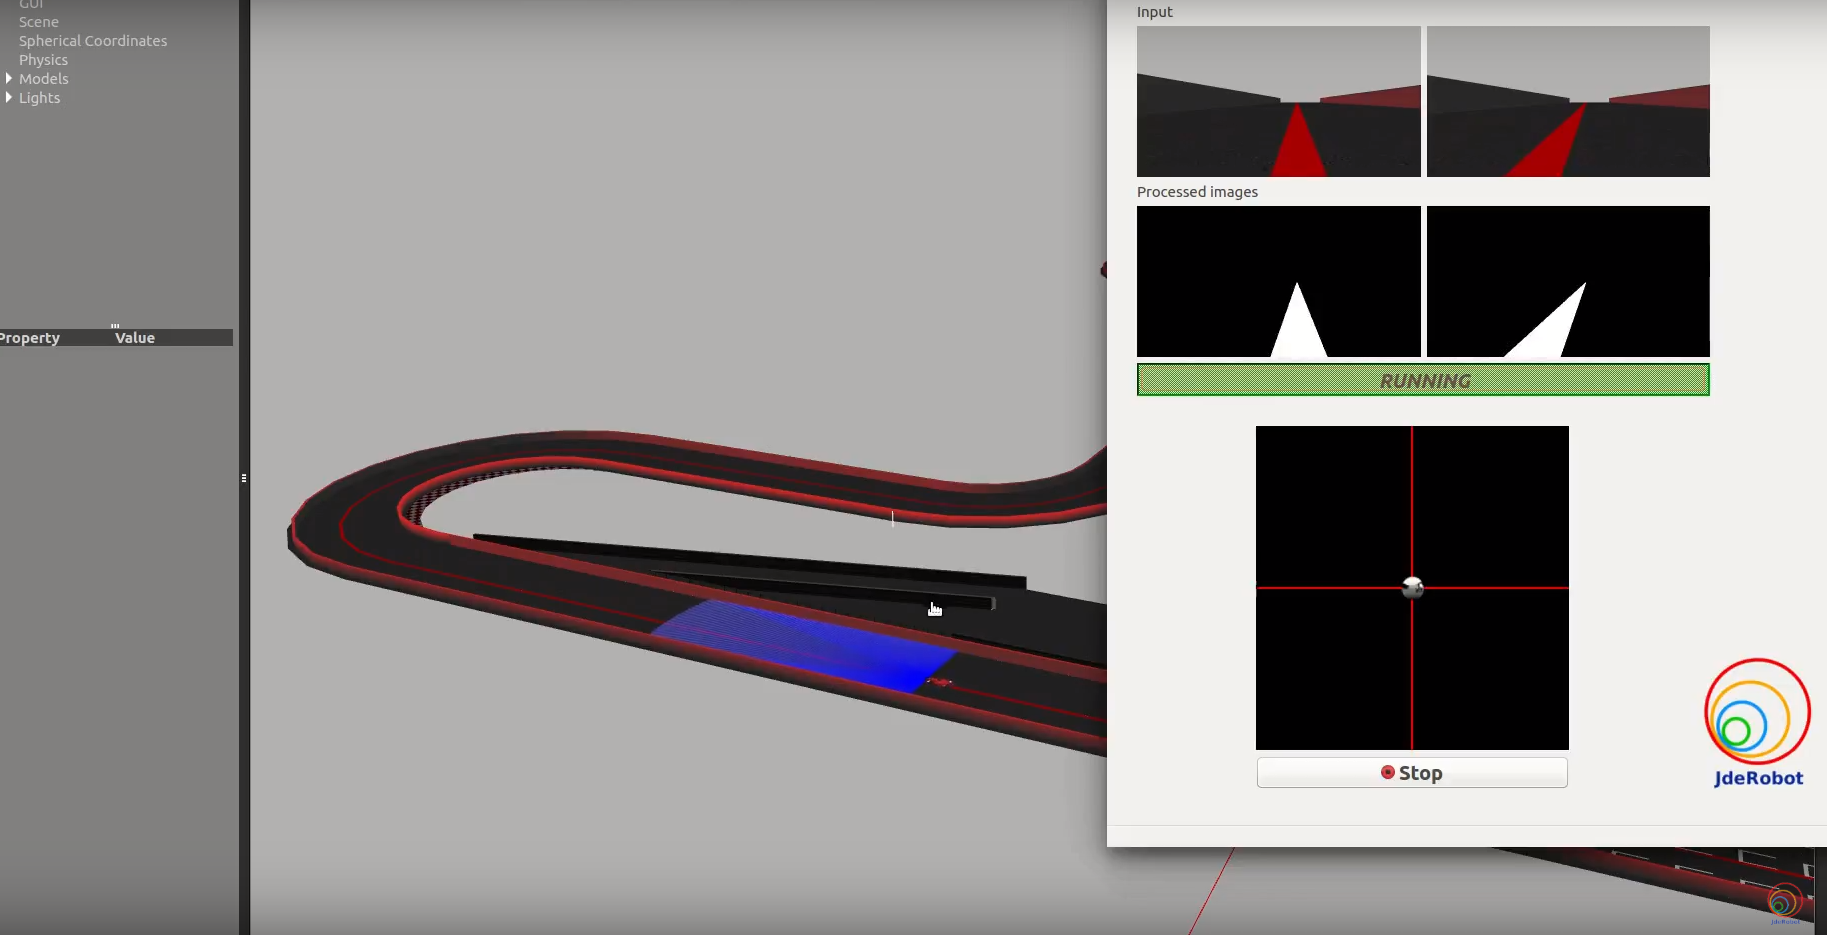
\includegraphics[width=0.95\textwidth]{figures/followline.png}
		\caption{Ejercicio ``Follow Line''}
		\label{fig.followline}
		\end{center}
\end{figure}

Este ejercicio \textit{Follow Line} (Figura \ref{fig.followline}) trata de un robot coche Fórmula1 que consta de una cámara en su parte frontal por la que recoge imágenes. En su código se deben recoger las imágenes y procesarlas de manera que filtre la línea roja del circuito y la siga hasta que complete el circuito por completo \footnote{\url{https://youtu.be/QGO9oaoBVoA}}.

\begin{figure}[H]
  \begin{center}
    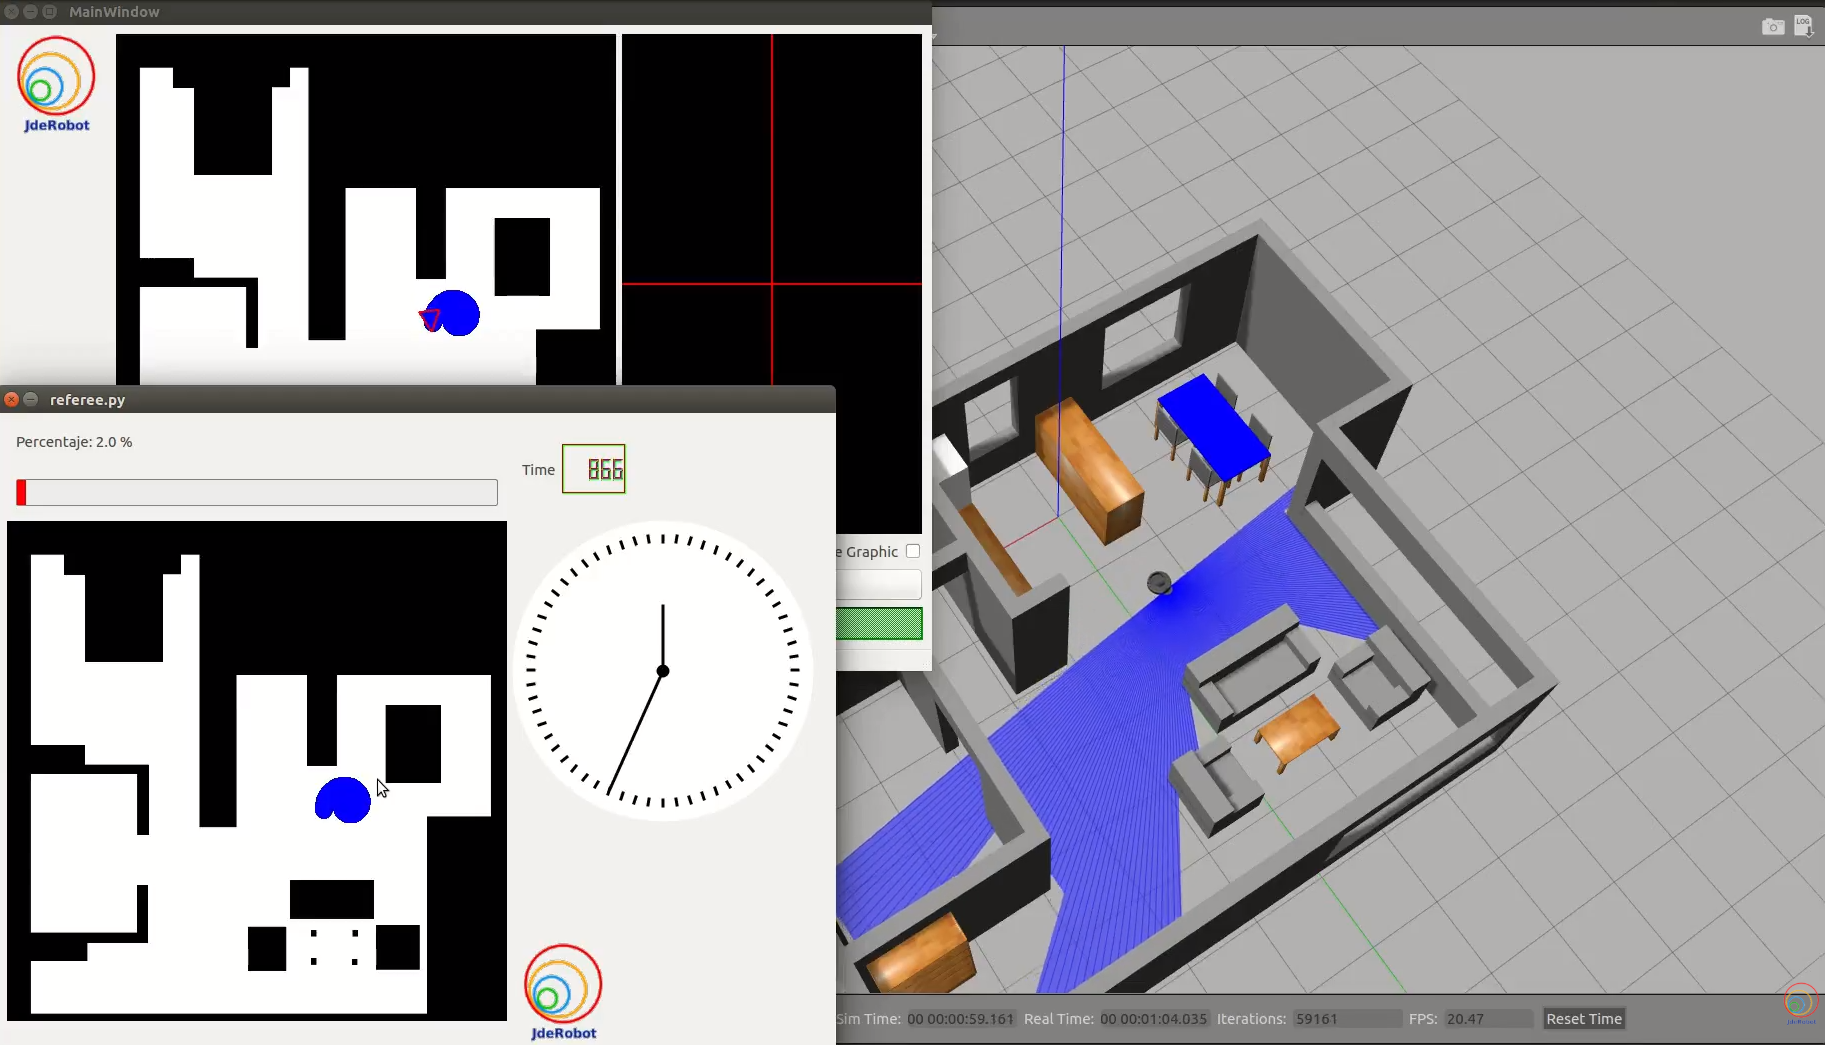
\includegraphics[width=0.95\linewidth, height=7cm]{figures/vacuumcleaner.png}
		\caption{Ejercicio de la aspiradora robótica}
		\label{fig.vacuumcleaner}
		\end{center}
\end{figure}

En este ejercicio \textit{Vacuum Cleaner} (Figura \ref{fig.vacuumcleaner}), el alumno debe recoger los datos del láser incluido en el modelo del robot aspiradora Roomba para que pase por el mayor área posible del escenario evitando la colisión con los obstáculos contenidos \footnote{\url{https://youtu.be/12muuY9JXLk}}.

\begin{figure}[H]
  \begin{center}
    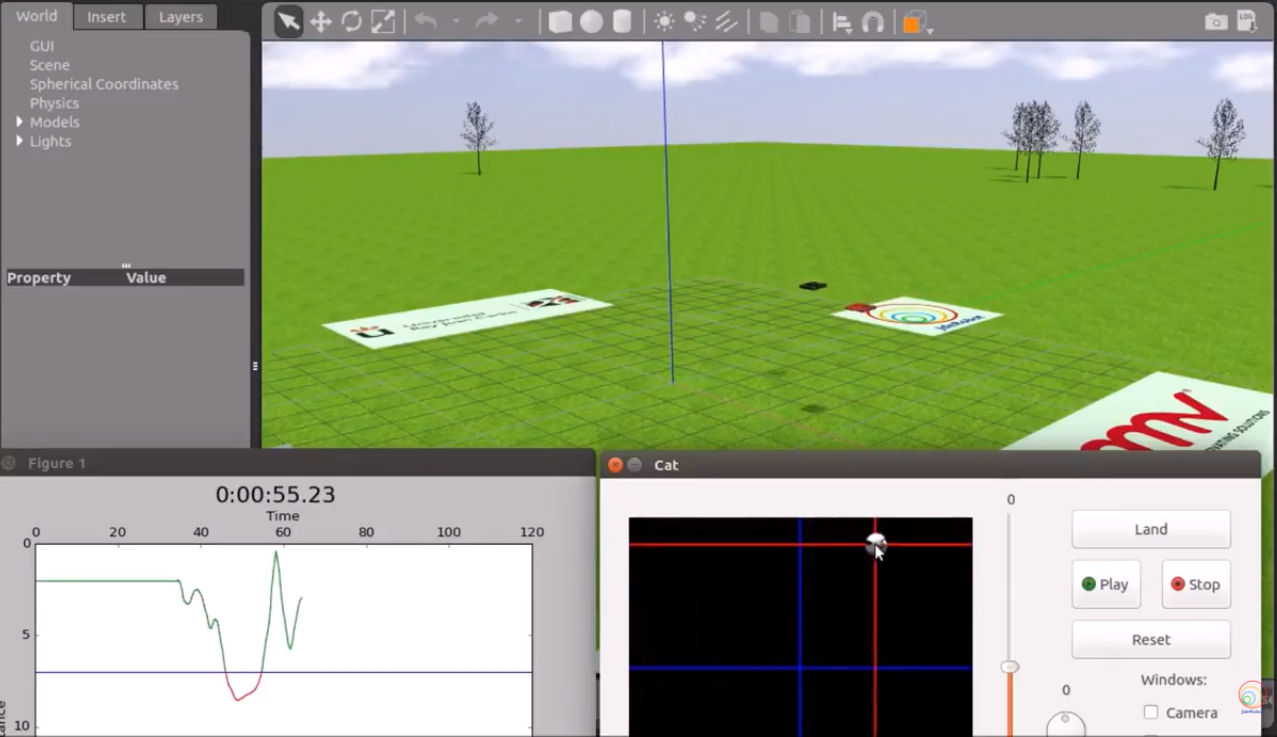
\includegraphics[width=0.95\textwidth, height=7.2cm]{figures/dronecatmouse.png}
		\caption{Ejercicio ``Drone-Cat-Mouse''}
		\label{fig.dronecatmouse}
		\end{center}
\end{figure}

\textit{Drone-Cat-Mouse} es una de las prácticas más complejas del entorno Robotics-Academy. En ella el alumno debe dotar de la lógica necesaria a un dron (dron negro) para recoger las imágenes captadas por su cámara y filtrarlas para encontrar y perseguir a un dron rojo. Una vez reconocido el dron rojo debe comandar al dron negro para perseguirlo dado que el rojo está en movimiento. El objetivo es que el dron negro se acerque los más posible al rojo, pero sin colisionar con él, emulando el juego Gato-Ratón\footnote{\url{https://www.youtube.com/watch?v=DYD9oPawhWg}}. Esta práctica se ha utilizado en las tes ediciones del campeonato \textit{Program-A-Robot}, la primera en la URJC, la segunda en las Jornadas Nacionales de Robótica y la tercera en la conferencia internacional IROS\footnote{\url{https://www.iros2018.org/competitions}}.

El contexto imediato de este Trabajo de Fin de Grado consiste en los ejercicios elaborados recientemente para enriquecer el contenido del entorno Robotics-Academy. Entre ellos cabe destacar el TFG de Irene López Rodríguez \textit{"Nuevas Prácticas en el Entorno Docente de Robótica Robotics-Academy"}\cite{tfg1} en el que se introdujeron dos prácticas nuevas llamadas ``Coche autónomo negociando un cruce'' y ``Aspiradora autónoma con autolocalización''. El primer ejercicio trata sobre un coche autónomo que llega a un cruce por el que circulan coches. El coche debe filtrar las imágenes para reconocer una señal de Stop, así como los coches que circulan en la carretera transversal y las líneas de los carriles. Cuando no detecte ningún coche circulando debe tomar la intersección y escoger el carril correcto. La segunda práctica de este TFG es similar a la práctica \textit{Vacuum Cleaner} pero consta del mapa con el escenario y sensor de posición, de manera que la aspiradora sabe en qué lugar del escenario se encuentra y no debe repetir áreas ya limpiadas.

Otro TFG destacado es el de Vanessa Fernández Martínez \textit{{“Nuevas Prácticas en el Entorno Docente de Robótica Robotics-Academy”}}\cite{tfg2}, en el cual se añadieron dos prácticas nuevas llamadas Aspiradora Autónoma o \textit{Vacuum Cleaner} y Aparcamiento Automático, además de mejorar la práctica Tele Taxi con nuevos modelos, un mejor rendimiento del algoritmo GPP de navegación global y la inclusión de un evaluador automático capaz de medir el desempeño del algoritmo y proporcionar una nota. La segunda práctica, llamada \textit{Autopark}, tiene como objetivo el aparcamiento de un coche autónomo mediante mediciones láser de los sensores frontales, laterales y posteriores.

También hay que mencionar el Trabajo de Fin de Grado desarrollado por Carlos Awadallah Estévez \textit{“Nuevas Prácticas Docentes de Robótica en el  Entorno JdeRobot-Academy”}\cite{tfg3}, en el cual se incorporan dos nuevas prácticas al entorno Robotics-Academy. La primera de ellas, llamada \textit{Follow Face}, trata de dar la lógica necesaria a una cámara pantilt de manera que procese las imágenes captadas por la cámara y reconozca la cara. Una vez hecho esto debe seguir el movimiento de la cara. La segunda práctica que se desarrolla en este TFG se llama \textit{Laser Loc}, en la cual mediante mediciones de los sensores laser y un mapa con el escenario es capaz de realizar estimaciones de posición mediante movimiento y odometría.

\vspace{4cm}

El objetivo de este TFG es ampliar el número de prácticas que forman el entorno Robotics-Academy desarrollando dos nuevas prácticas, una completamente nueva y otra actualizada y adaptada a \textit{ROS}, además de aportar en el elenco de prácticas en su versión de cuadernillos de Jupyter para acercar al entorno a dar soporte multiplataforma.

En los próximos capítulos serán abordados los elementos necesarios para conseguir este objetivo. Comenzaremos con el Capítulo 2, en el que se concretarán los objetivos marcados, así como el punto de partida de este TFG y la metodología que ha sido empleada. En la Capítulo 3 se abordará la infraestructura utilizada para realizar el proyecto. En los Capítulos 4 y 5 explicaremos las dos prácticas que se han abordado en este TFG. Y, por último, en el Capítulo 6, se expondrán las conclusiones obtenidas, además de las posibles líneas de mejora futuras.

